\begin{appendices}

\chapter{Experiment Set-Up}
\label{app:method}


\chapter{PCA Results}
\label{app:PCA_res_full}

\chapter{List of Tested Plastic}
\label{app:list_plast}




\begin{figure}
    \centering
    \includegraphics[height = 9cm, angle = 90]{Images/order.png}
    \caption{List of microplastics - state, class, additives and application}
    \label{fig:order}
\end{figure}




\begin{comment}
\begin{center}
\begin{adjustbox}{angle=90}
\begin{tabular}{ |c|l|l|l|l| } 
 \hline
 \textbf{Ref Number} & \textbf{State} & \textbf{Class} & \textbf{Additives} & \textbf{Application}\\ 
 \hline
CRT131.00 & Post-Industrial Recyclate Pellets & PE: LDPE/LLDPE & Colorants, Printing inks & Extrusion, sheet\\
CRT150.00 & Post-Consumer Recyclate Regrind & PE-HD & Colorants & Injection moulding, crates\\
CRT170.00 & Environmental Pellets & PE: LDPE/HDPE & Unspecified Additives & Waste, beached pellets\\
CRT171.00 & Environmental Fragments (Regrind) & PE-HD & Unspecified Additives & Waste, beached fish box yellow\\
CRT200.00 & Pristine Pellets & PP-Homopolymer & Stabilizers & Extrusion, injection moulding\\
CRT250.00 & Post Consumer Recyclate: Pellets & PP Mixture & Unspecified Additives & Mainly Injection Moulding\\
CRT300.00 & Pristine Pellets & PS General purpose & Unknown & Extrusion blending, packaging\\
CRT331.00 & Post Consumer Recyclate Regrind & PS Mixture & Unspecified Additives & Plant Trays Outdoor\\ 
CRT400.00 & Pristine Pellets & PET Amorphous & No intentionally additives & Blow moulding \& extrusion sheet\\
CRT451.00 & Post Consumer Recyclate Regrind & PET Amorphous & No intentionally additives & Blow moulding \& extrusion sheet\\
CRT500.00 & Pellets & PVC Soft & Softener & Injection moulding \& extrusion\\
CRT530.00 & Pellets & PVC Hard & Softener \& Mineral Filler & Injection moulding \& extrusion\\
 \hline
\end{tabular}
\end{adjustbox}
\end{center}
\end{comment}

\chapter{Images of Tested Plastic Samples}
\label{app:image_plast}


\chapter{Plots of Signatures}
\label{app:signatures}

\begin{figure}
    \centering
    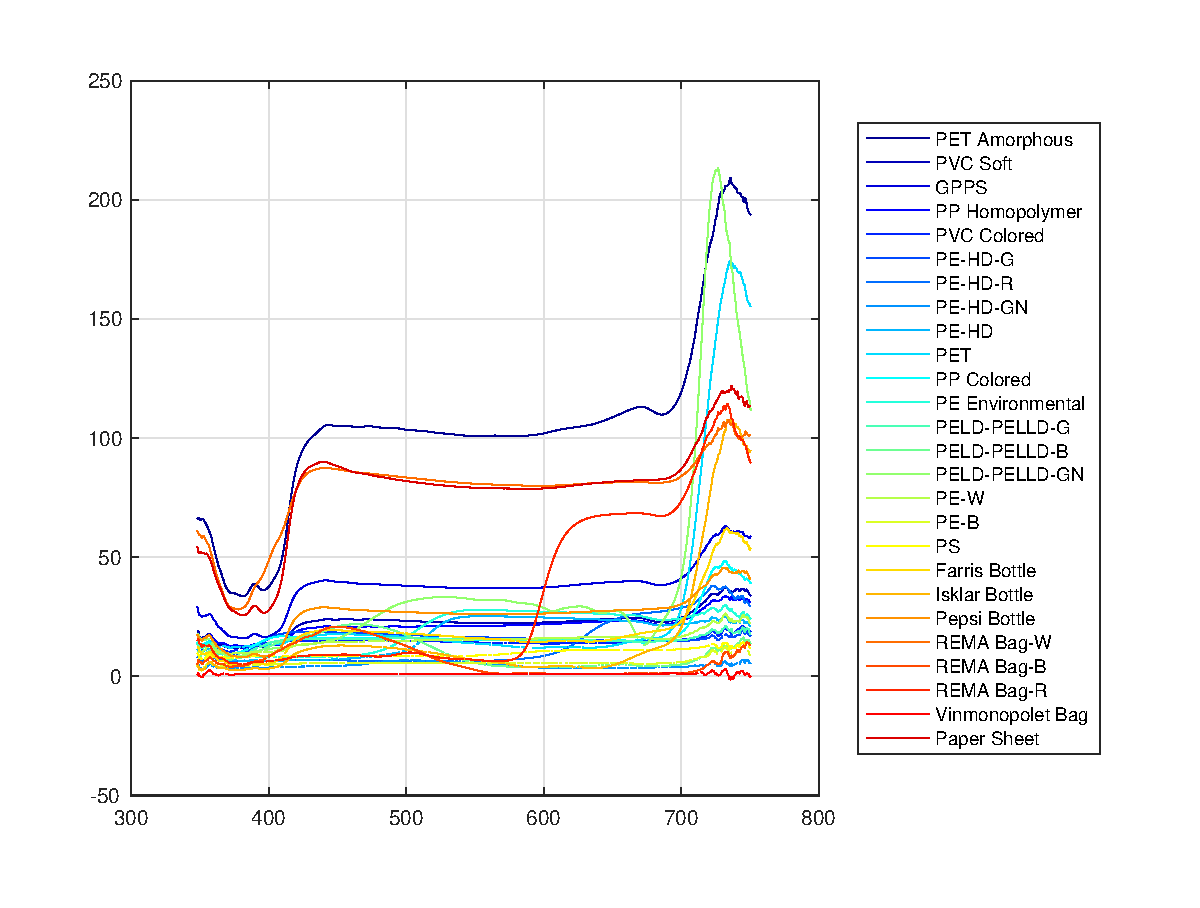
\includegraphics[width = 12cm]{Images/appendix/All.eps}
    \caption{All}
    \label{fig:all}
\end{figure}

\begin{figure}
    \centering
    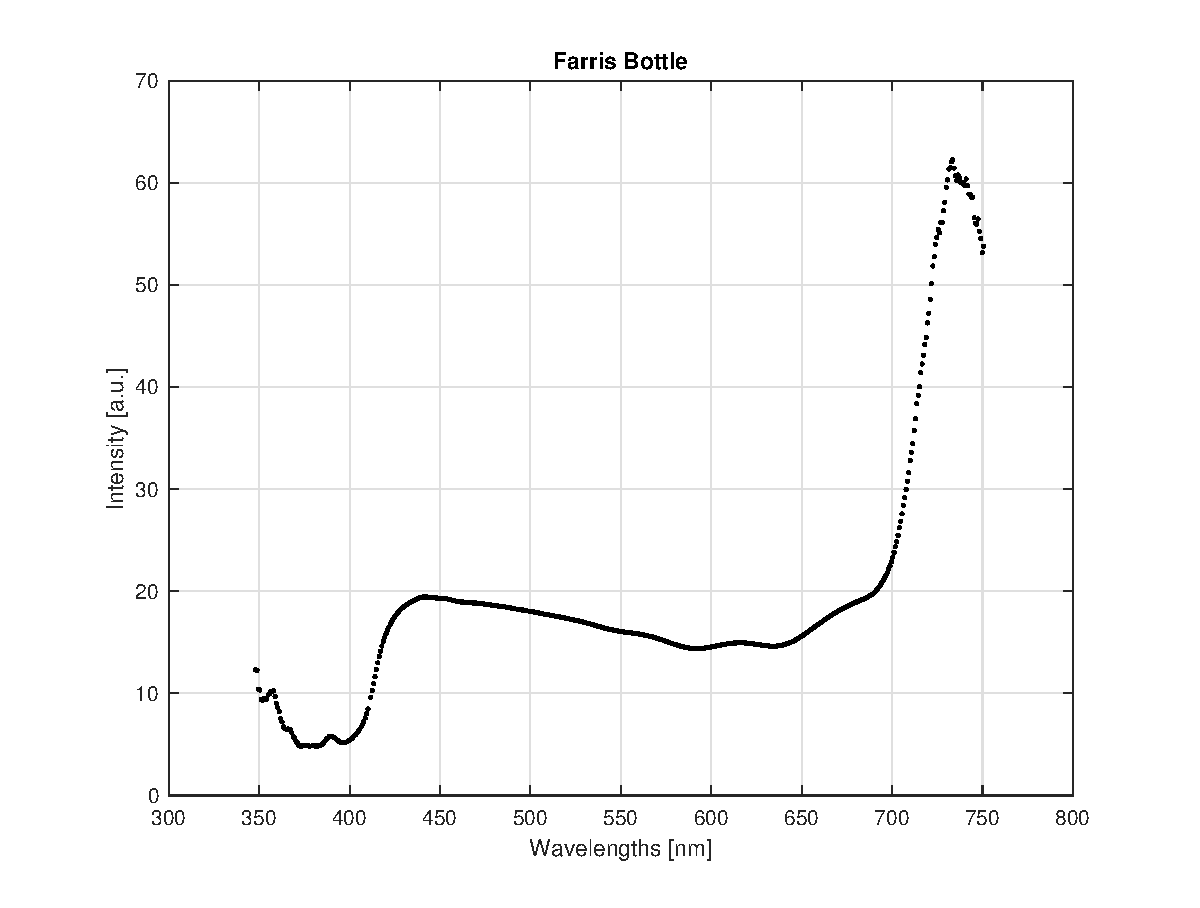
\includegraphics[width = 12cm]{Images/appendix/farris.eps}
    \caption{Farris}
    \label{fig:my_label}
\end{figure}

%DENNE FUNKER IKKE!?!
\begin{comment}
\begin{figure}
    \centering
    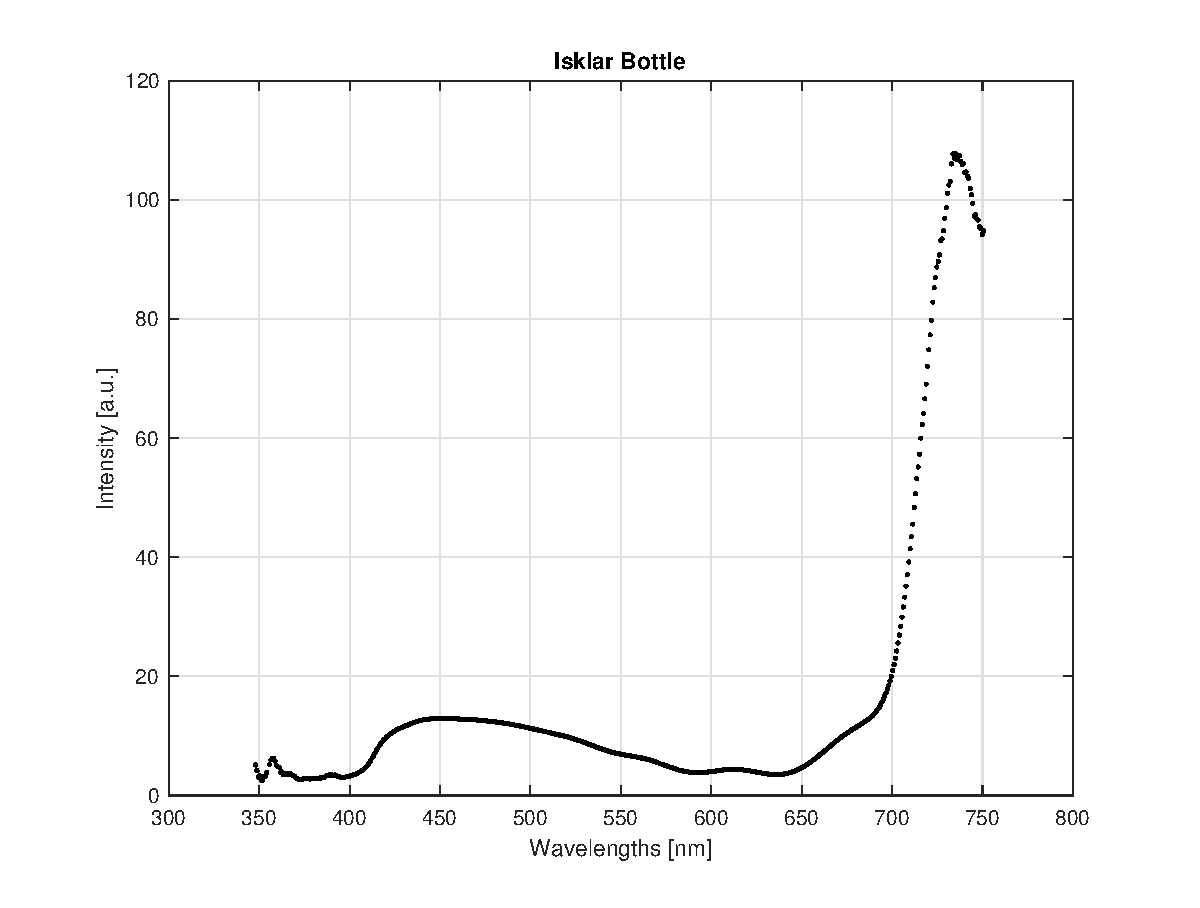
\includegraphics[width = 12cm]{Images/appendix/isklar(blue).eps}
    \caption{Isklar}
    \label{fig:isklar}
\end{figure}
\end{comment}

\begin{figure}
    \centering
    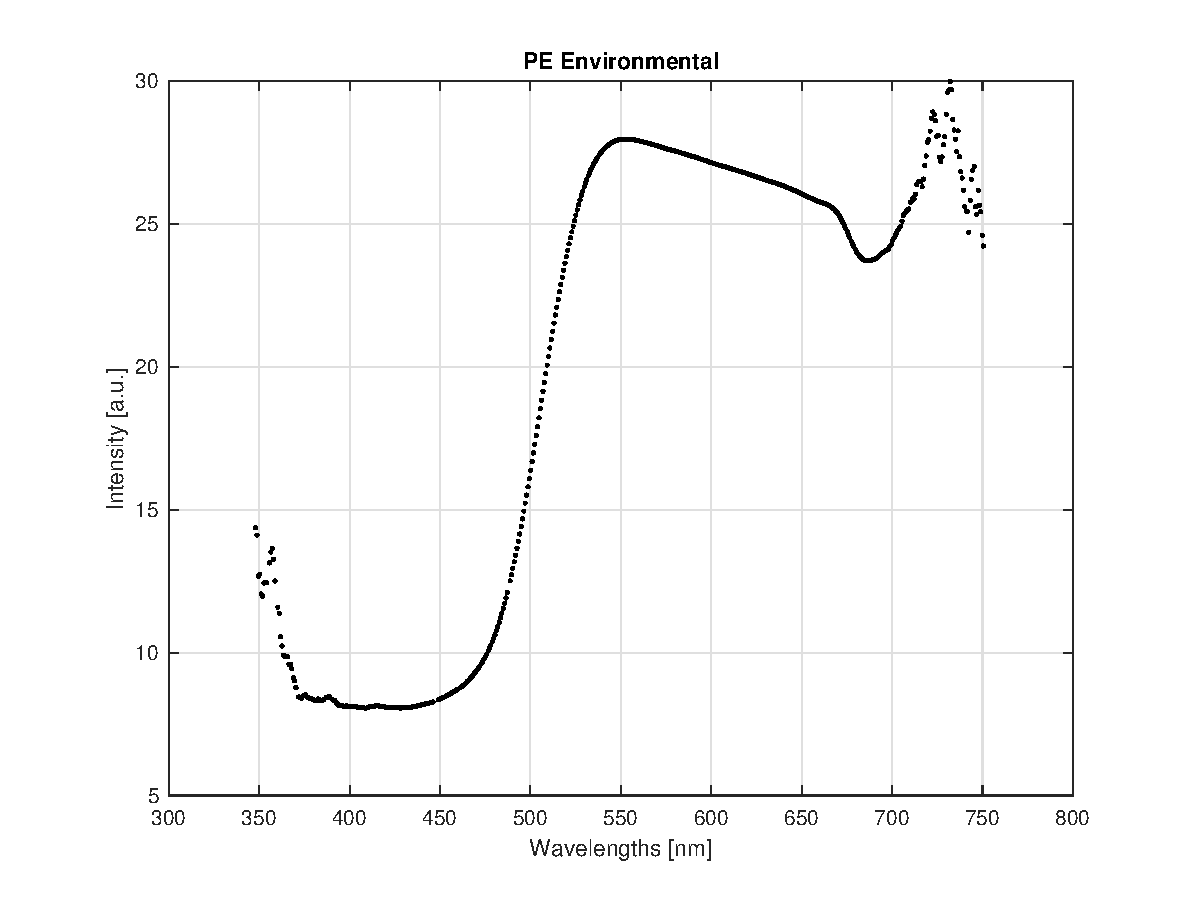
\includegraphics[width = 12cm]{Images/appendix/p-env_yellowbowl.eps}
    \caption{PE environmental (yellow fishbowl)}
    \label{fig:pe_env}
\end{figure}

\begin{figure}
    \centering
    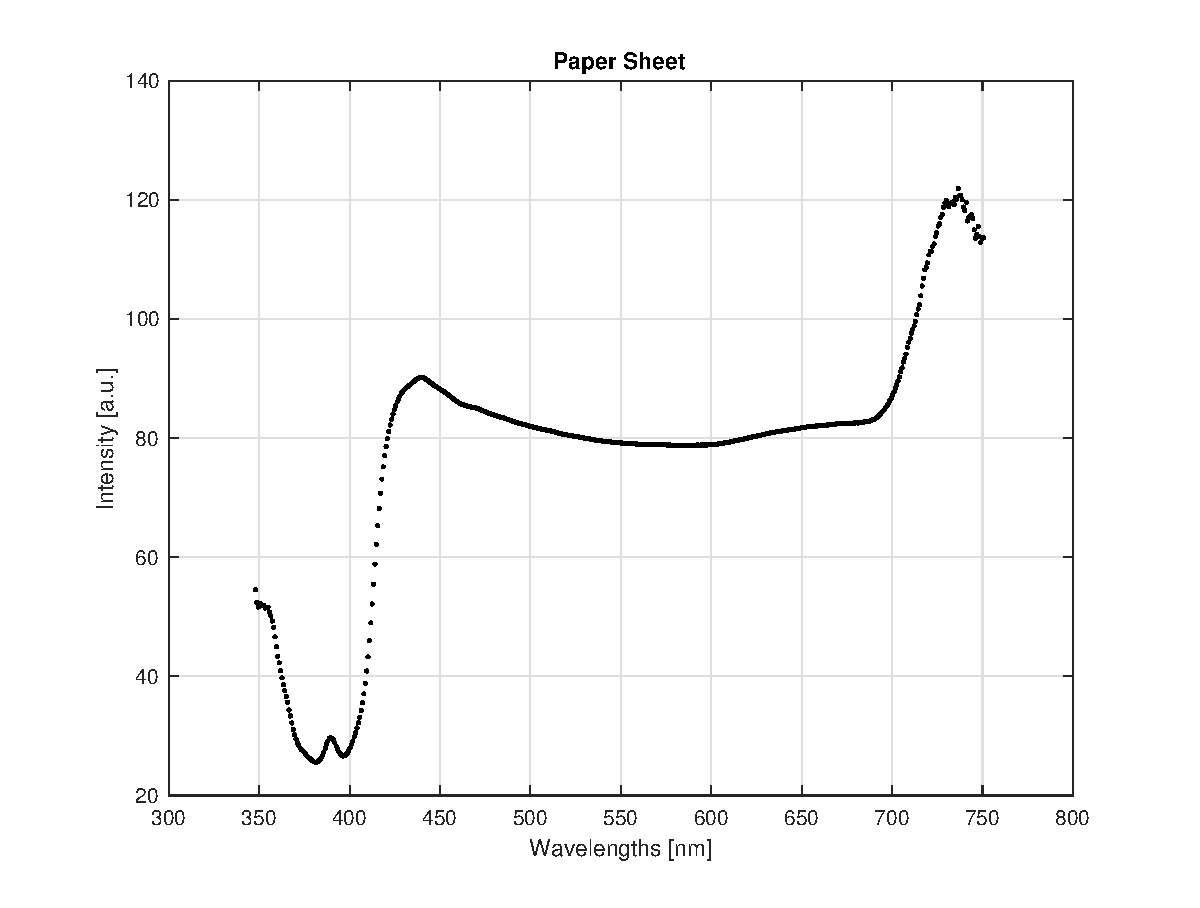
\includegraphics[width = 12cm]{Images/appendix/papersheet.eps}
    \caption{Paper sheet}
    \label{fig:paper}
\end{figure}

\begin{figure}
    \centering
    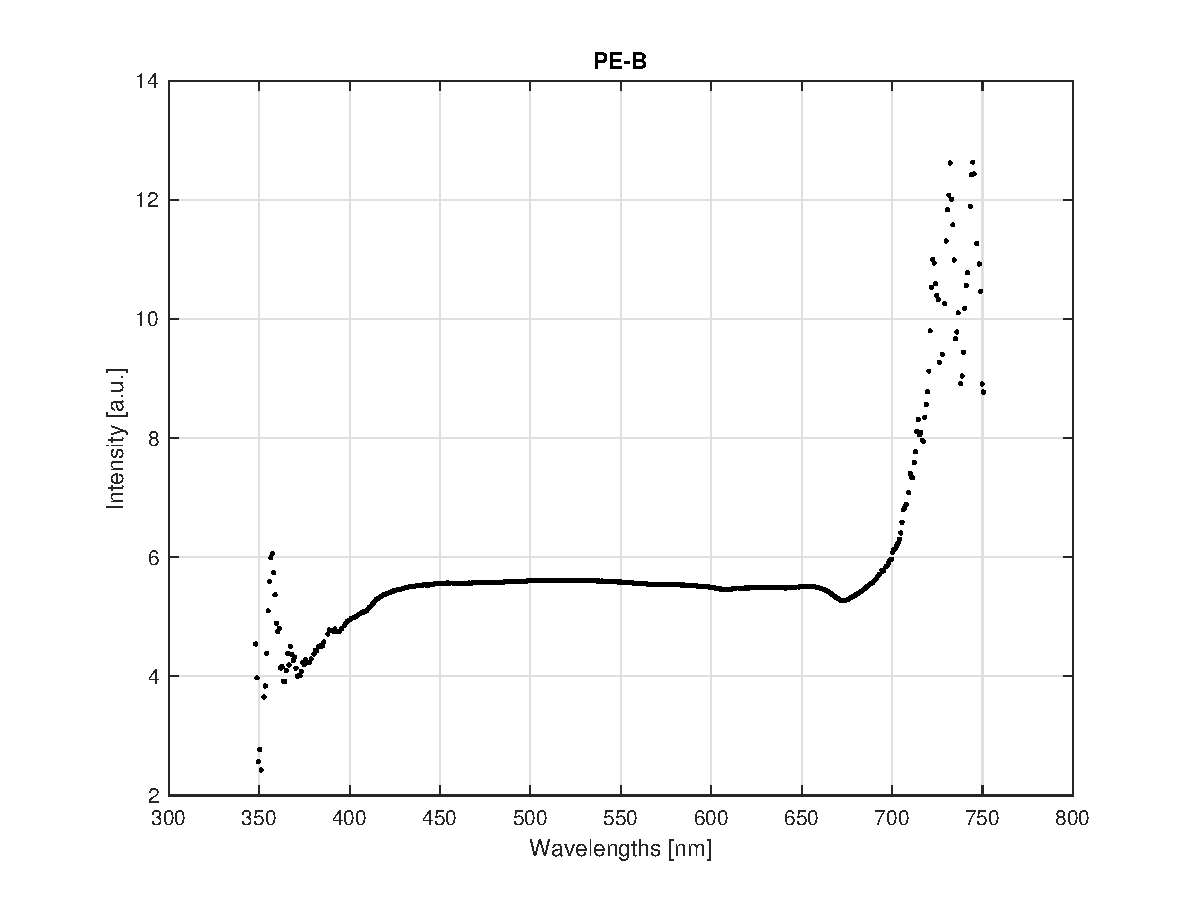
\includegraphics[width = 12cm]{Images/appendix/pe-beach-black.eps}
    \caption{PE beach-pellets, black}
    \label{fig:pe_beach_b}
\end{figure}

\begin{figure}
    \centering
    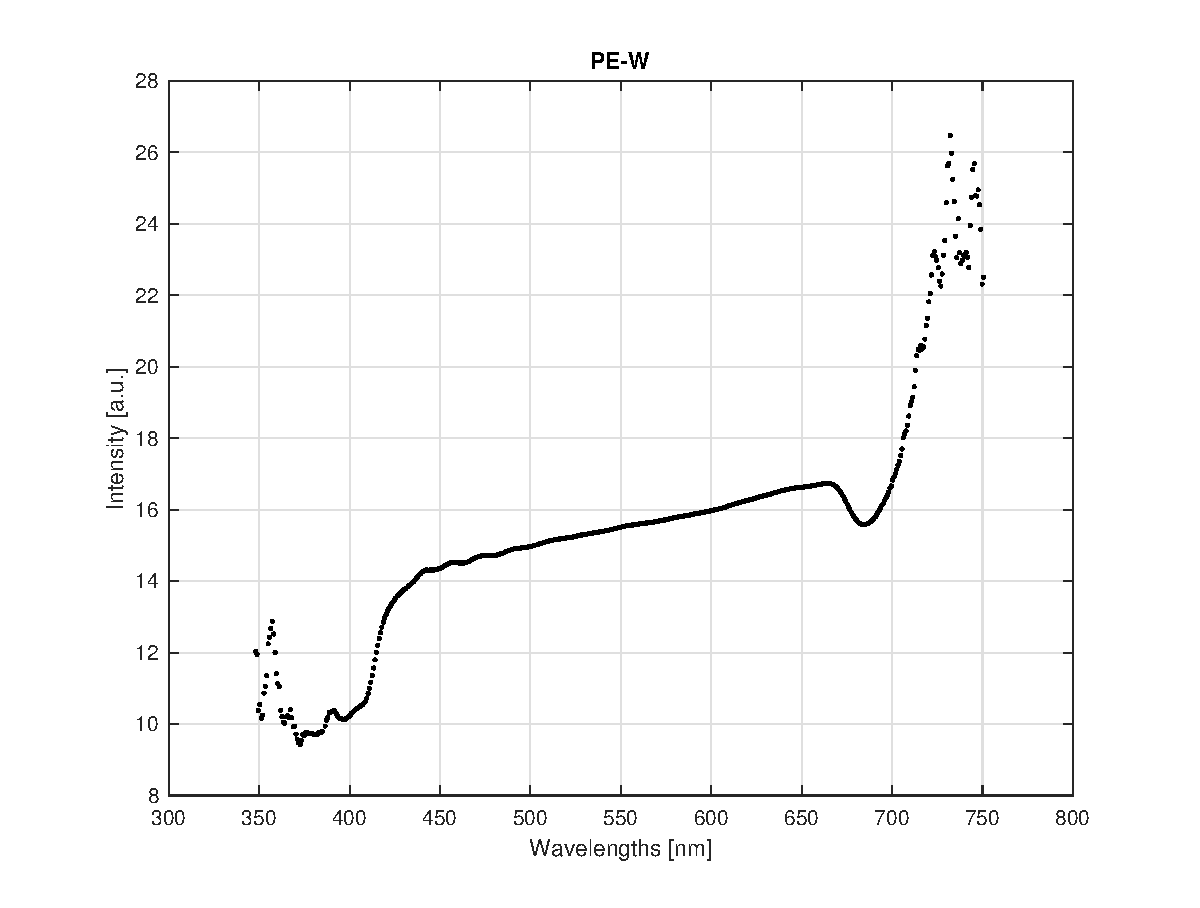
\includegraphics[width = 12cm]{Images/appendix/pe-beach-white.eps}
    \caption{PE beach-pellets, white}
    \label{fig:pe_beach_w}
\end{figure}

\begin{figure}
    \centering
    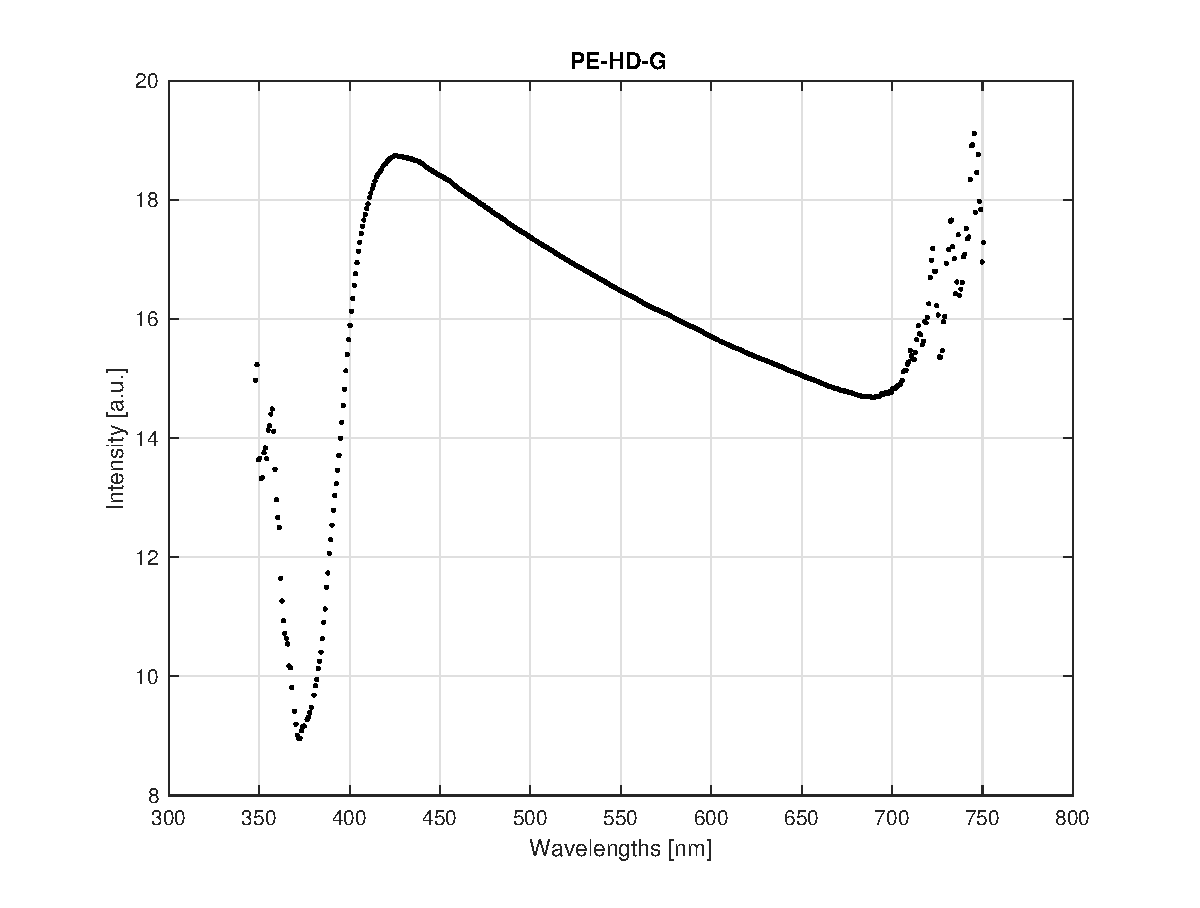
\includegraphics[width = 12cm]{Images/appendix/pe-hd-postconsum-gray.eps}
    \caption{PE-HD, Post Consumer, Gray}
    \label{fig:pehd-gray}
\end{figure}

\begin{figure}
    \centering
    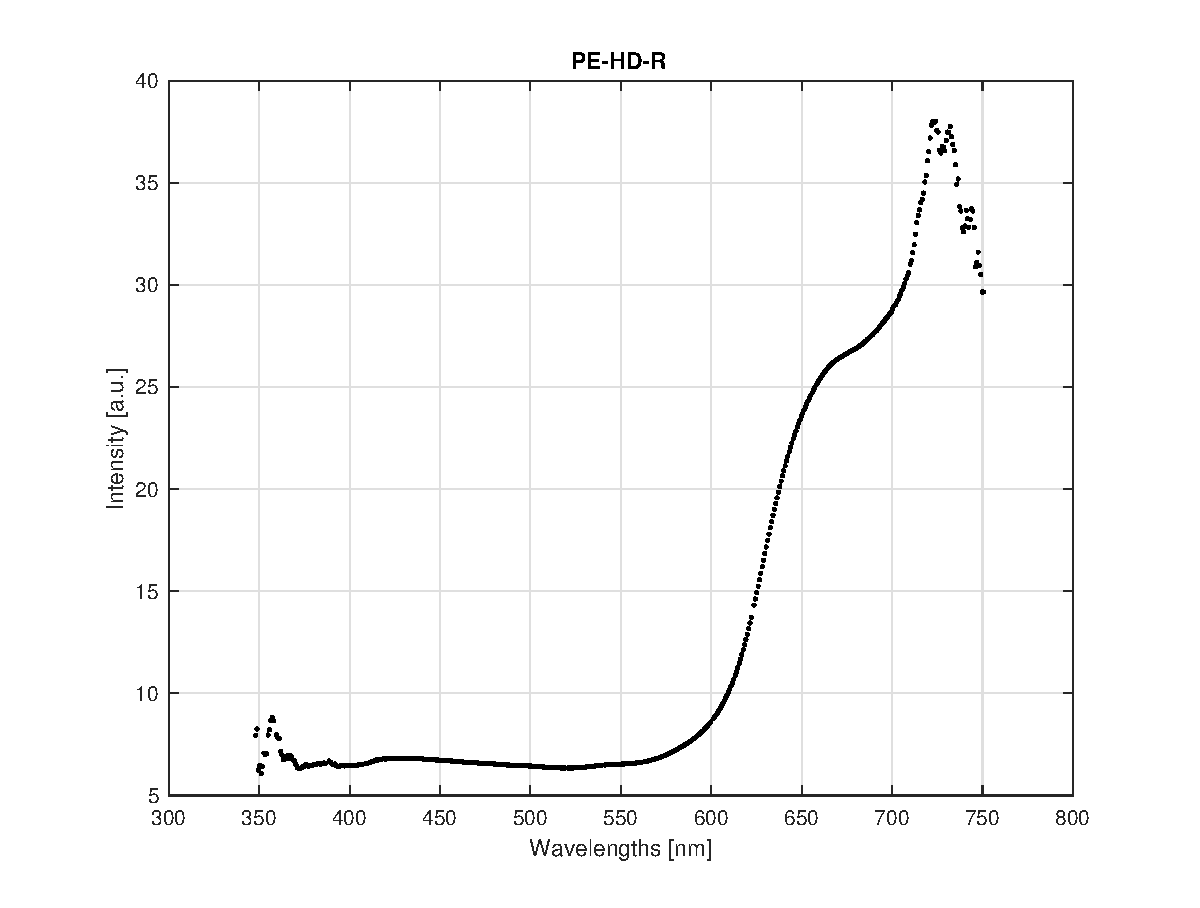
\includegraphics[width = 12cm]{Images/appendix/pe-hd-postconsum-red.eps}
    \caption{PE-HD, Post Consumer, Red}
    \label{fig:pehd-red}
\end{figure}

\begin{figure}
    \centering
    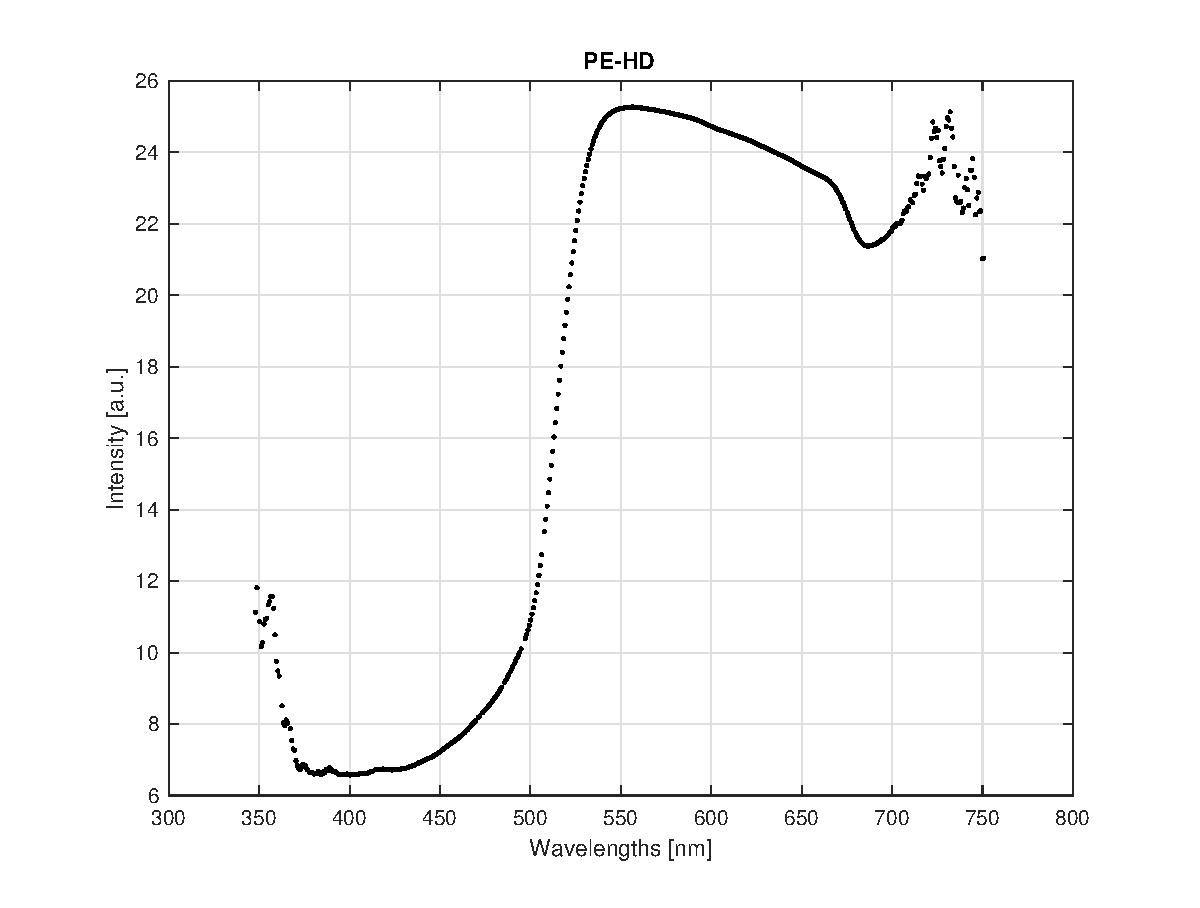
\includegraphics[width = 12cm]{Images/appendix/pe-hd-postconsum.eps}
    \caption{PE-HD, Post Consumer, Yellow}
    \label{fig:pehd-yellow}
\end{figure}

\begin{figure}
    \centering
    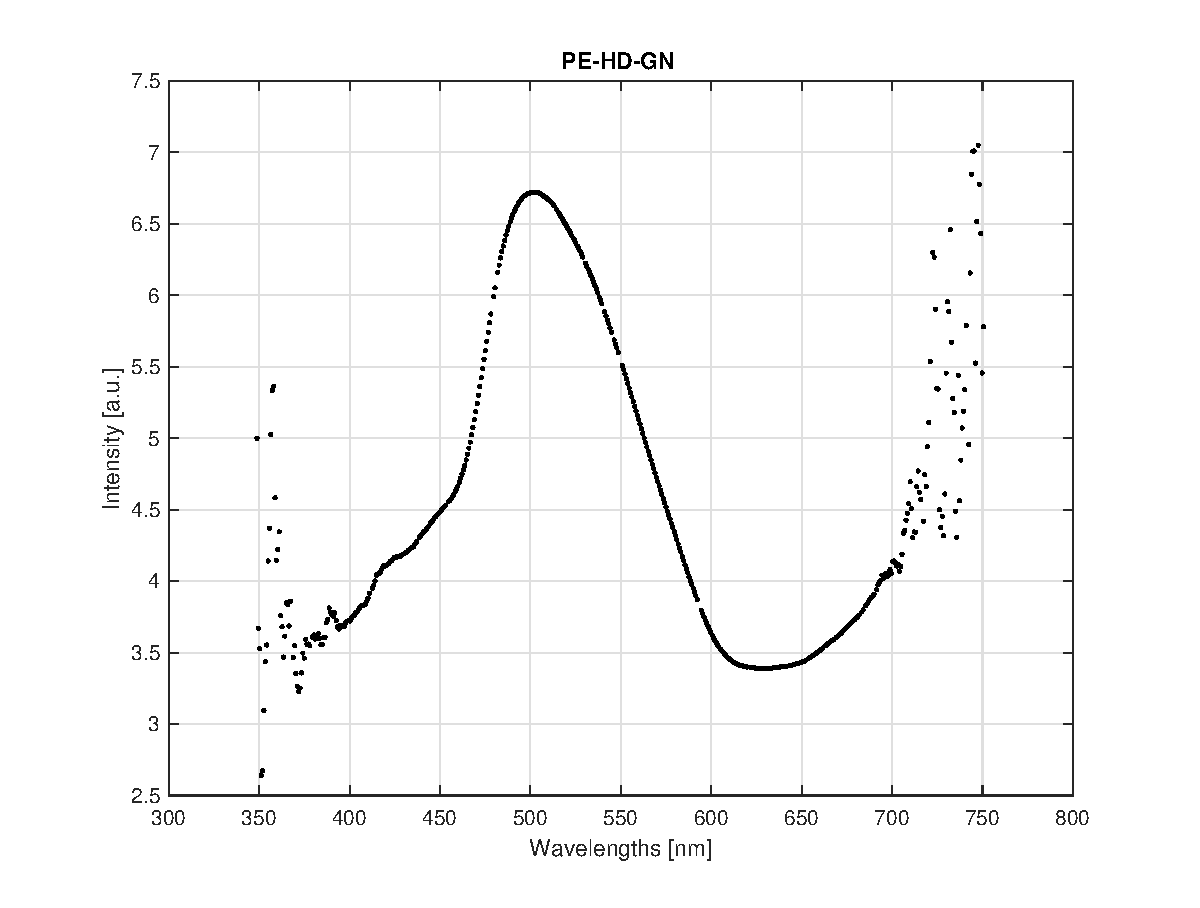
\includegraphics[width = 12cm]{Images/appendix/pe-hd-postconsumer-green.eps}
    \caption{PE-HD, Post Consumer, Green}
    \label{fig:pehd-green}
\end{figure}

\begin{figure}
    \centering
    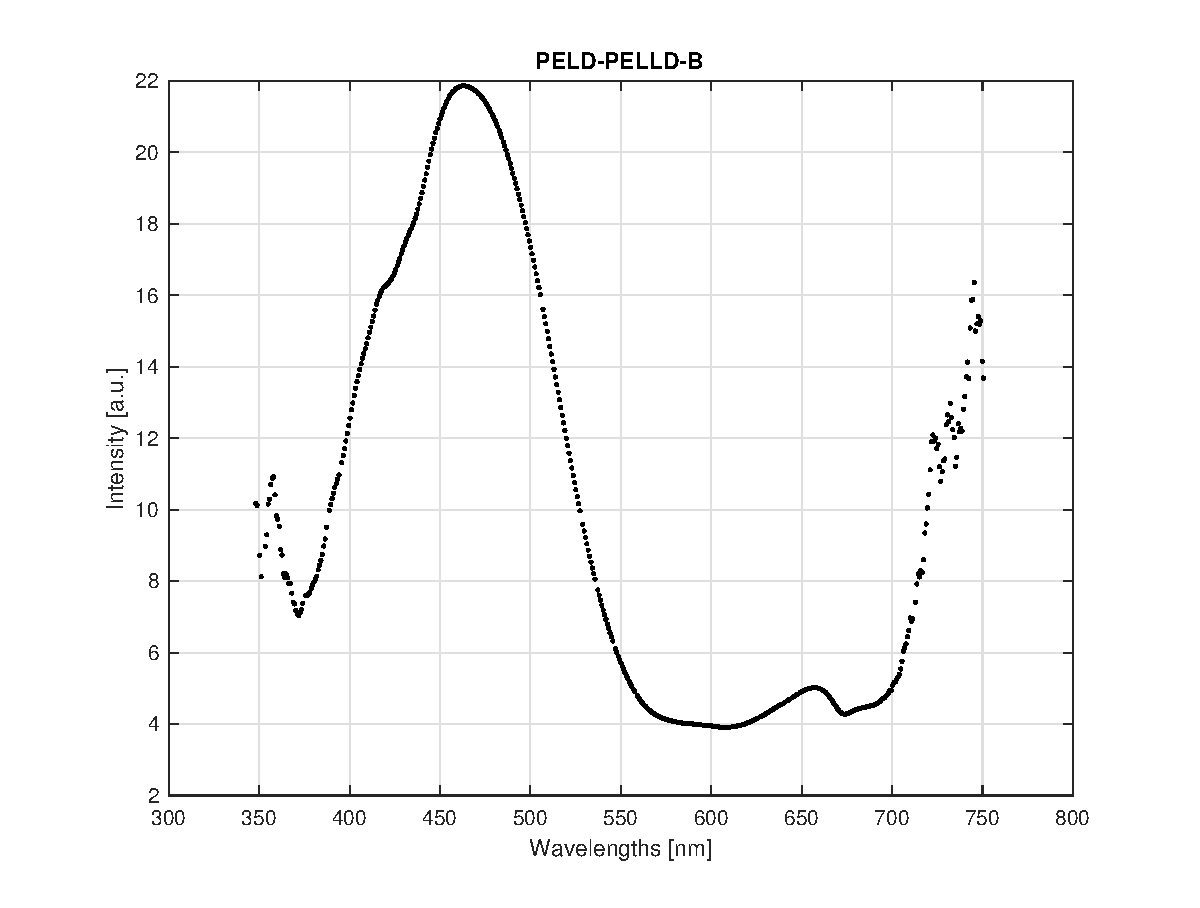
\includegraphics[width = 12cm]{Images/appendix/pe-ld-postindust-blue.eps}
    \caption{PE-LD, Post Industrial, Blue}
    \label{fig:peld-blue}
\end{figure}

\begin{figure}
    \centering
    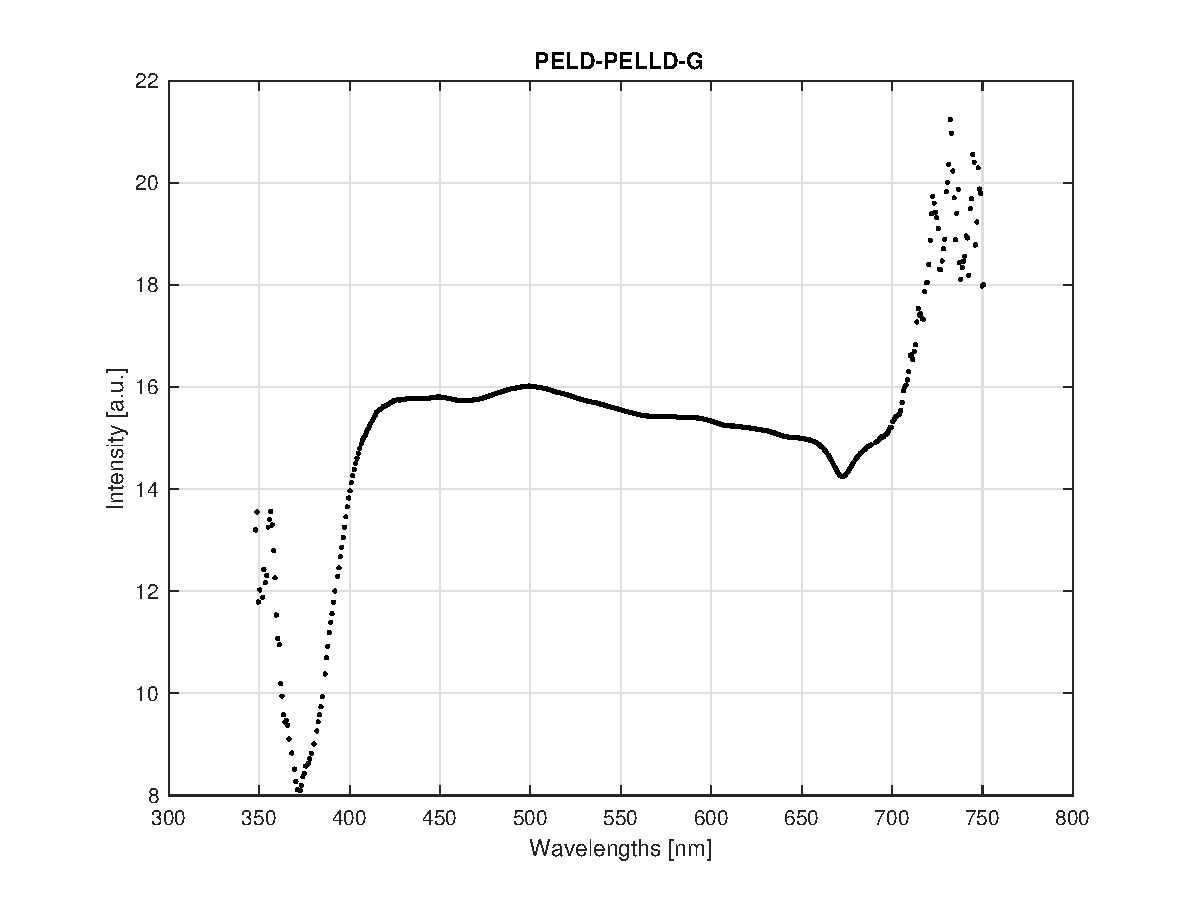
\includegraphics[width = 12cm]{Images/appendix/pe-ld-postindust-gray.eps}
    \caption{PE-LD, Post Industrial, Gray}
    \label{fig:peld-gray}
\end{figure}

\begin{figure}
    \centering
    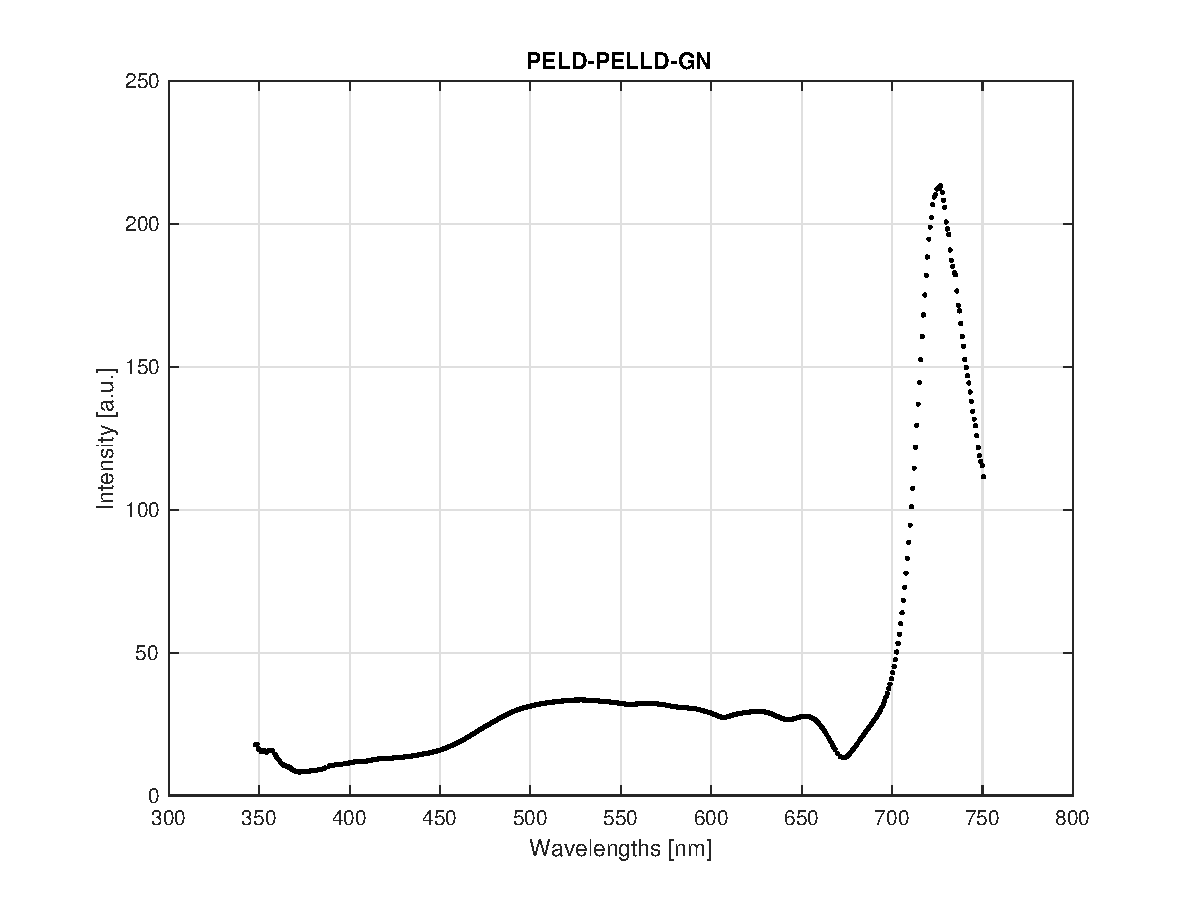
\includegraphics[width = 12cm]{Images/appendix/pe-ld-postindust-green.eps}
    \caption{PE-LD, Post Industrial, Green}
    \label{fig:peld-green}
\end{figure}

\begin{figure}
    \centering
    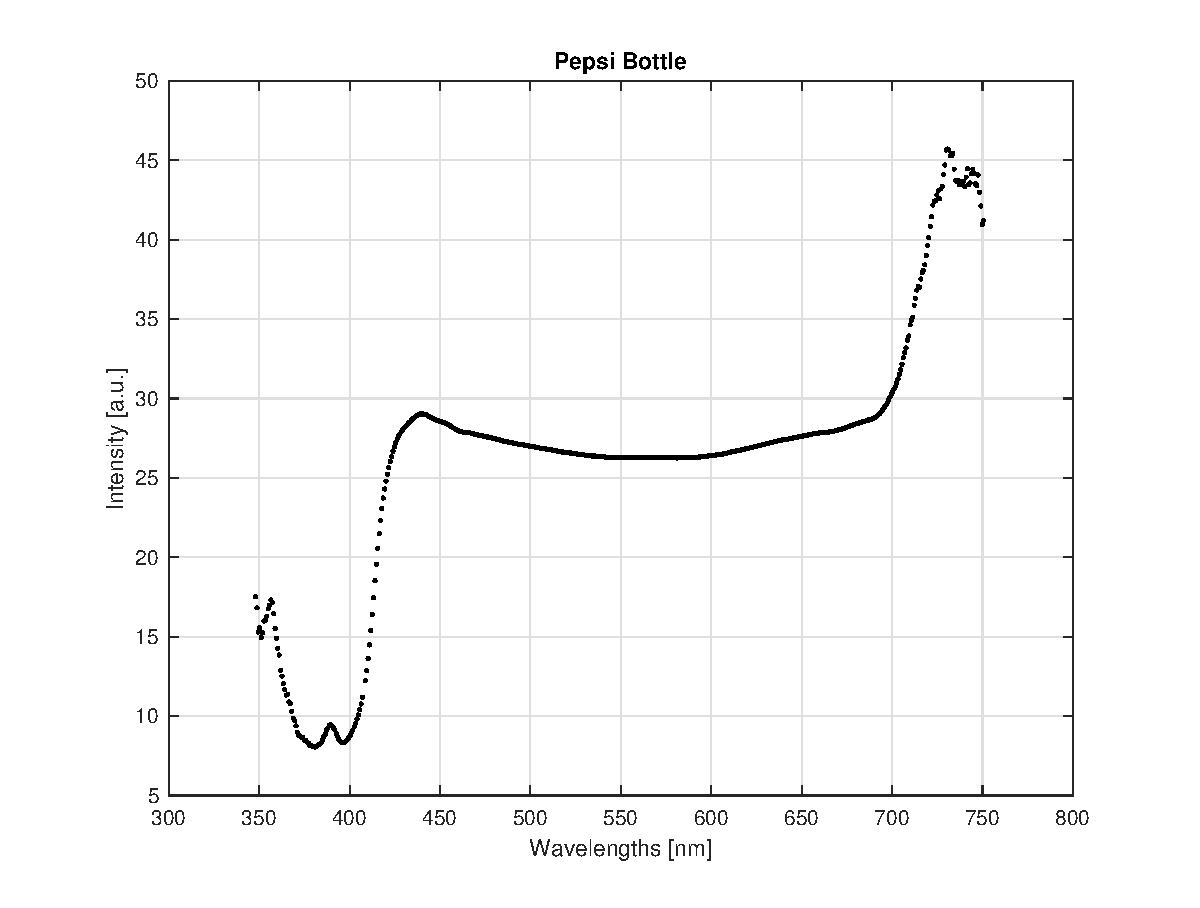
\includegraphics[width = 12cm]{Images/appendix/pepsi.eps}
    \caption{Pepsi}
    \label{fig:pepsi}
\end{figure}

\begin{figure}
    \centering
    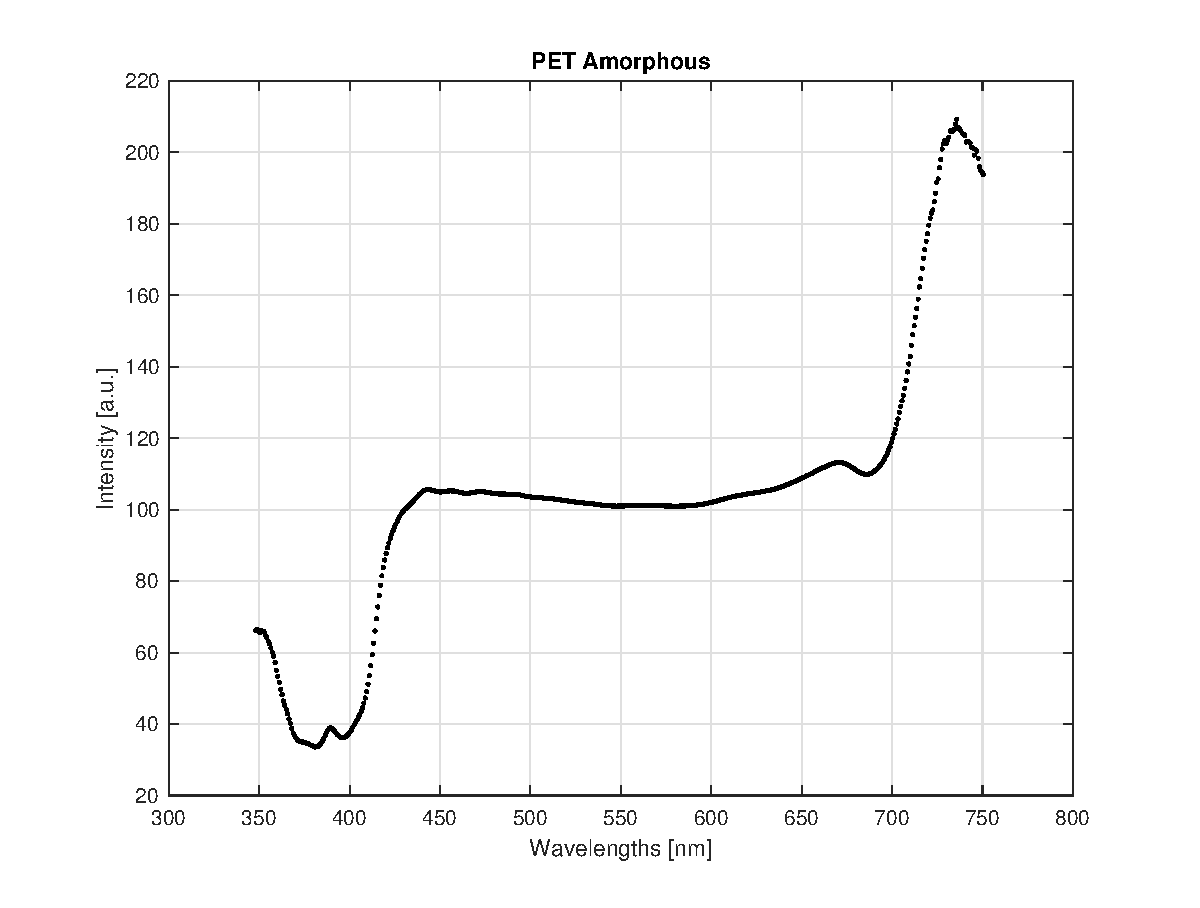
\includegraphics[width = 12cm]{Images/appendix/pet-amorphous-pristine-clear.eps}
    \caption{PET Amorphous, Clear}
    \label{fig:pet}
\end{figure}

\begin{figure}
    \centering
    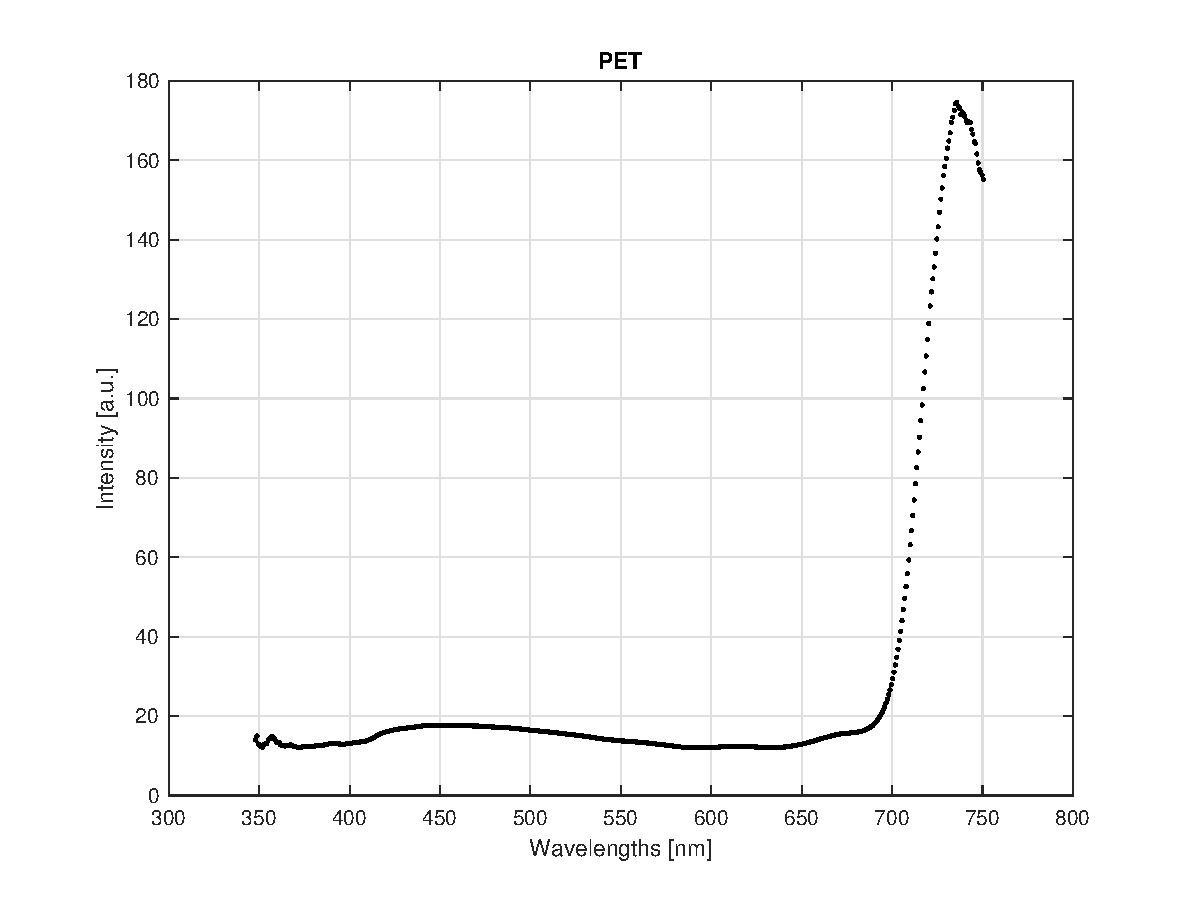
\includegraphics[width = 12cm]{Images/appendix/pet-postconsum.eps}
    \caption{PET Post Consumer, Clear}
    \label{fig:pet-pc}
\end{figure}

\begin{figure}
    \centering
    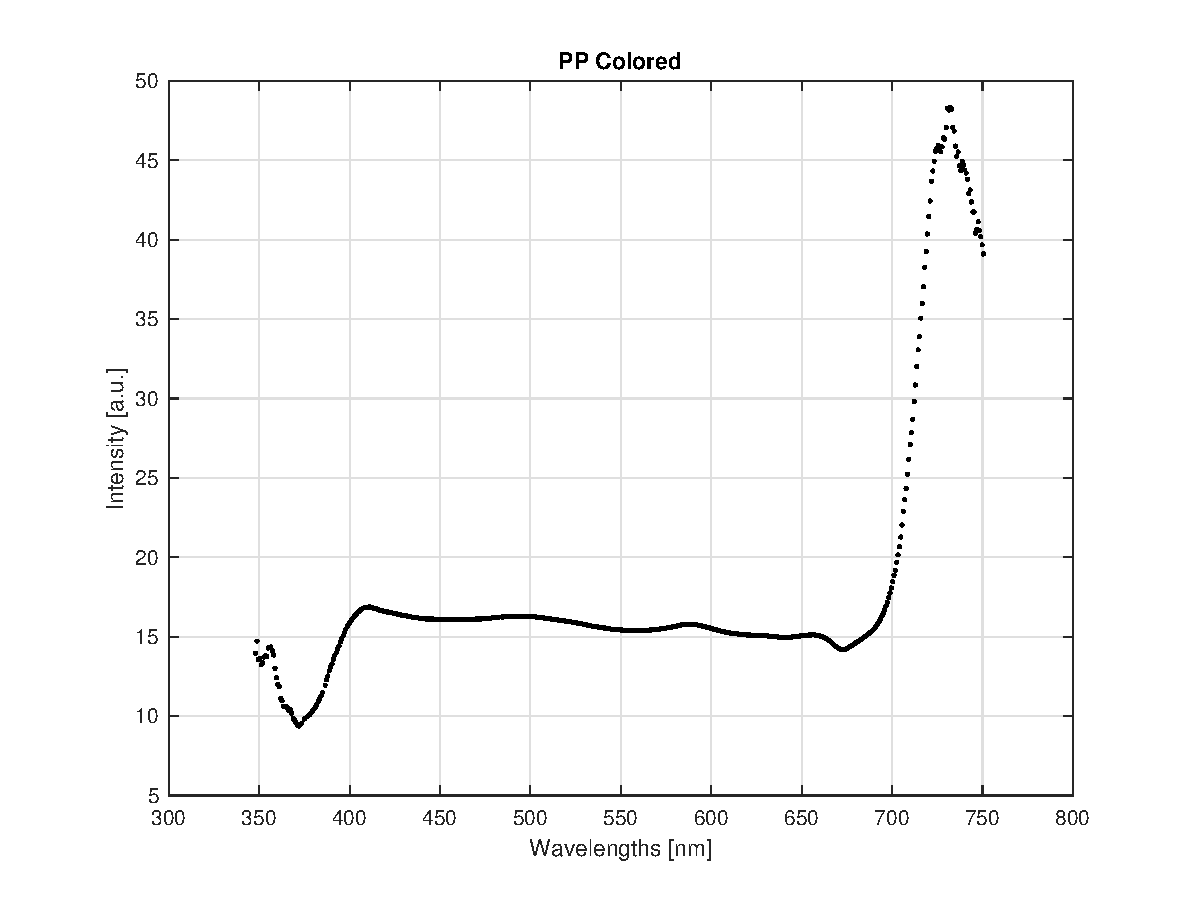
\includegraphics[width = 12cm]{Images/appendix/pp-postconsum-gray.eps}
    \caption{PP, Post Consumer, Gray}
    \label{fig:pp-gray}
\end{figure}

\begin{figure}
    \centering
    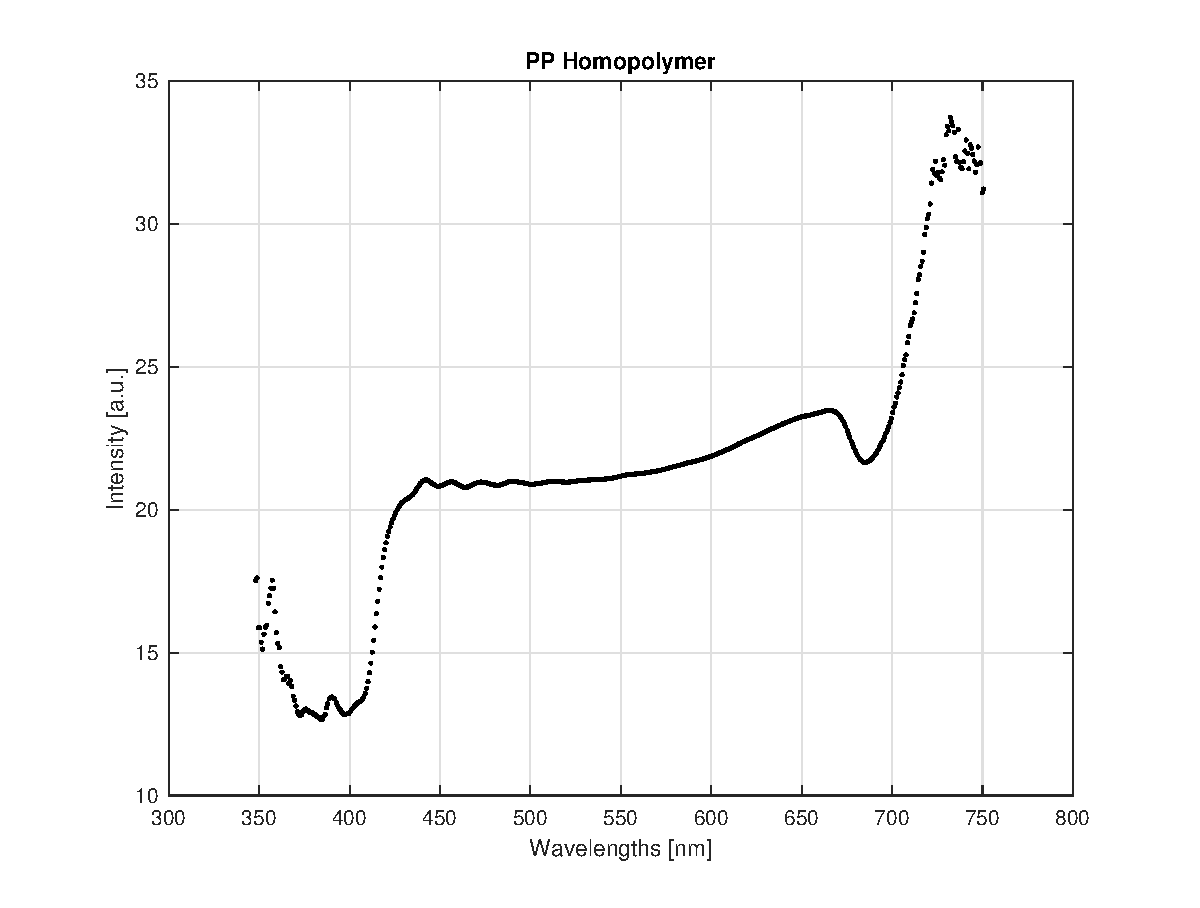
\includegraphics[width = 12cm]{Images/appendix/pp-pristine-clear.eps}
    \caption{PP, Pristine, Clear}
    \label{fig:pp-clear}
\end{figure}

\begin{figure}
    \centering
    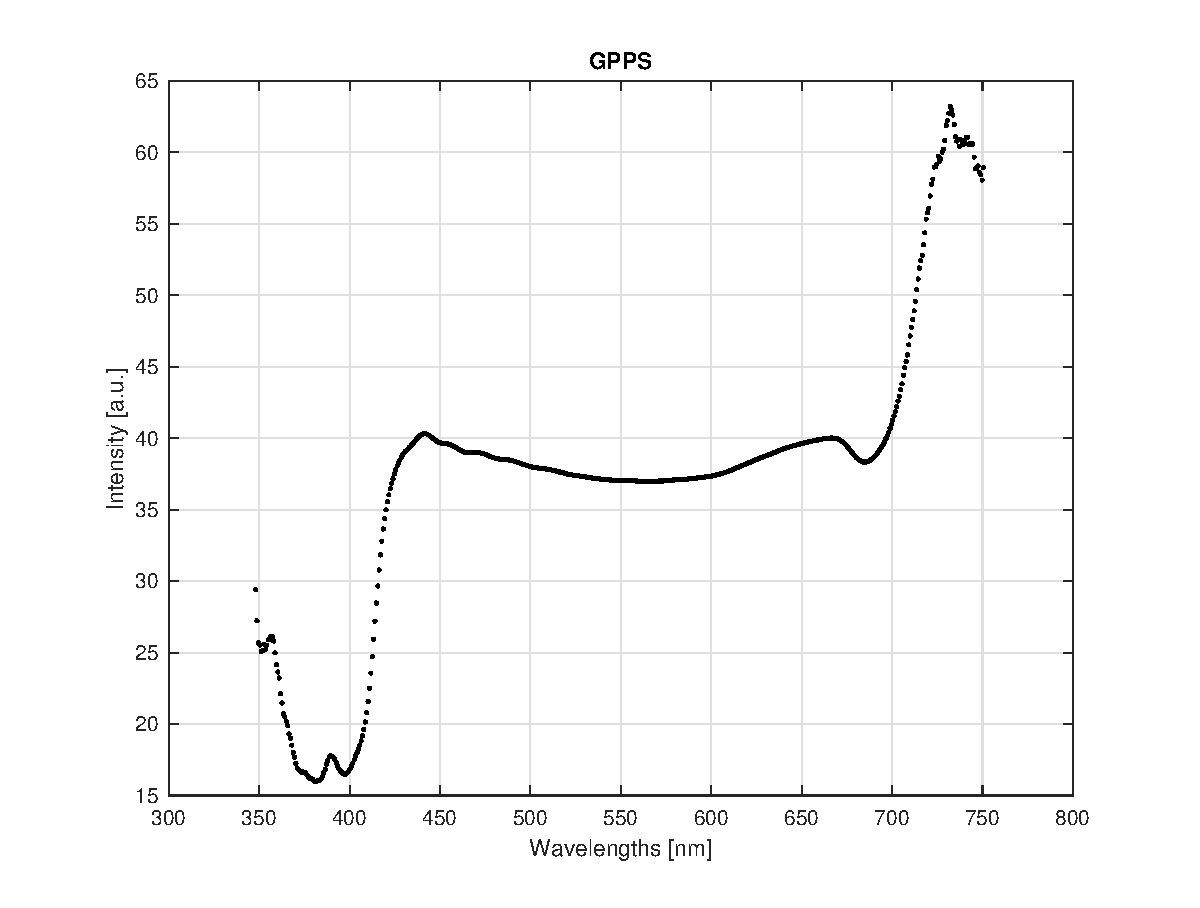
\includegraphics[width = 12cm]{Images/appendix/ps-pristine-clear.eps}
    \caption{PS, Pristine, Clear}
    \label{fig:ps-clear}
\end{figure}

\begin{figure}
    \centering
    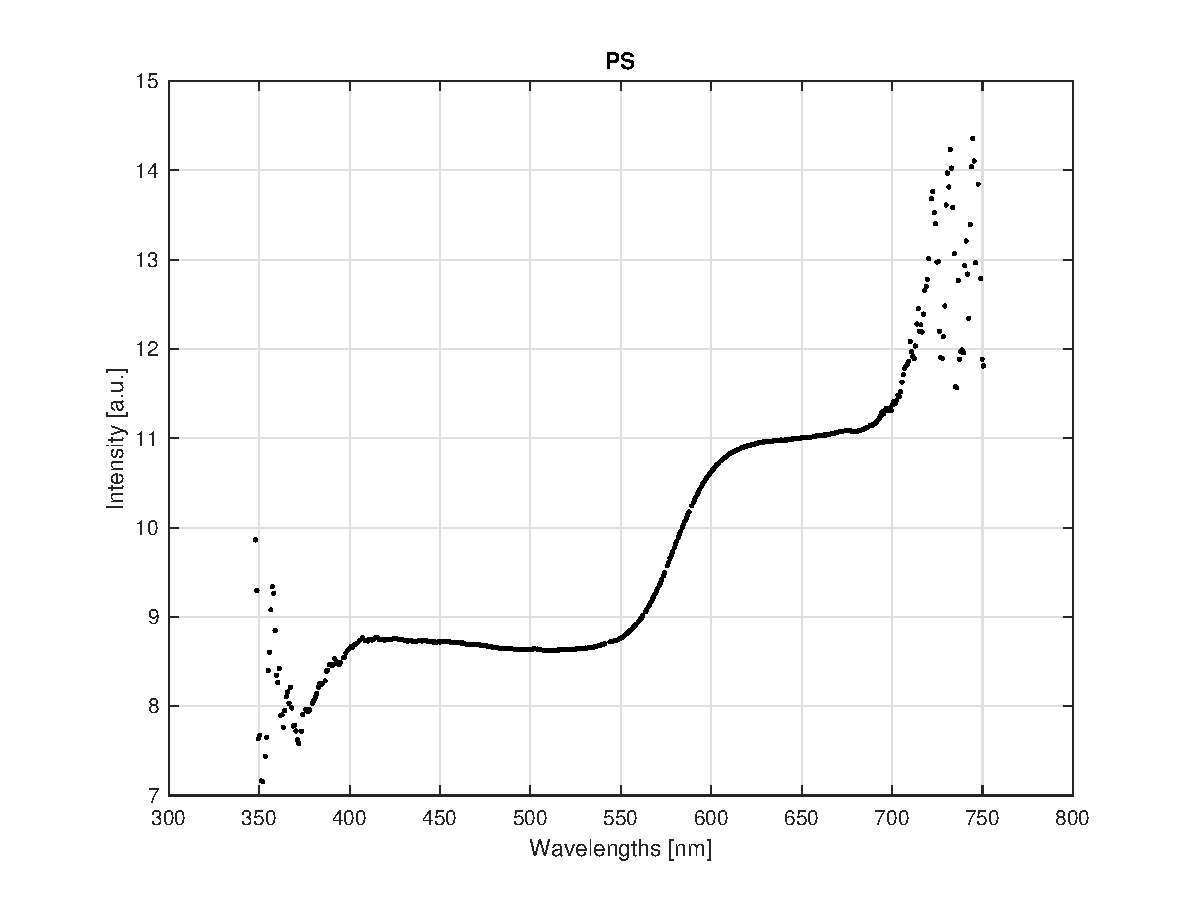
\includegraphics[width = 12cm]{Images/appendix/ps-postindust.eps}
    \caption{PS, Post Industrial, Looks like black/orange/white coffee powder}
    \label{fig:ps-coffee}
\end{figure}

\begin{figure}
    \centering
    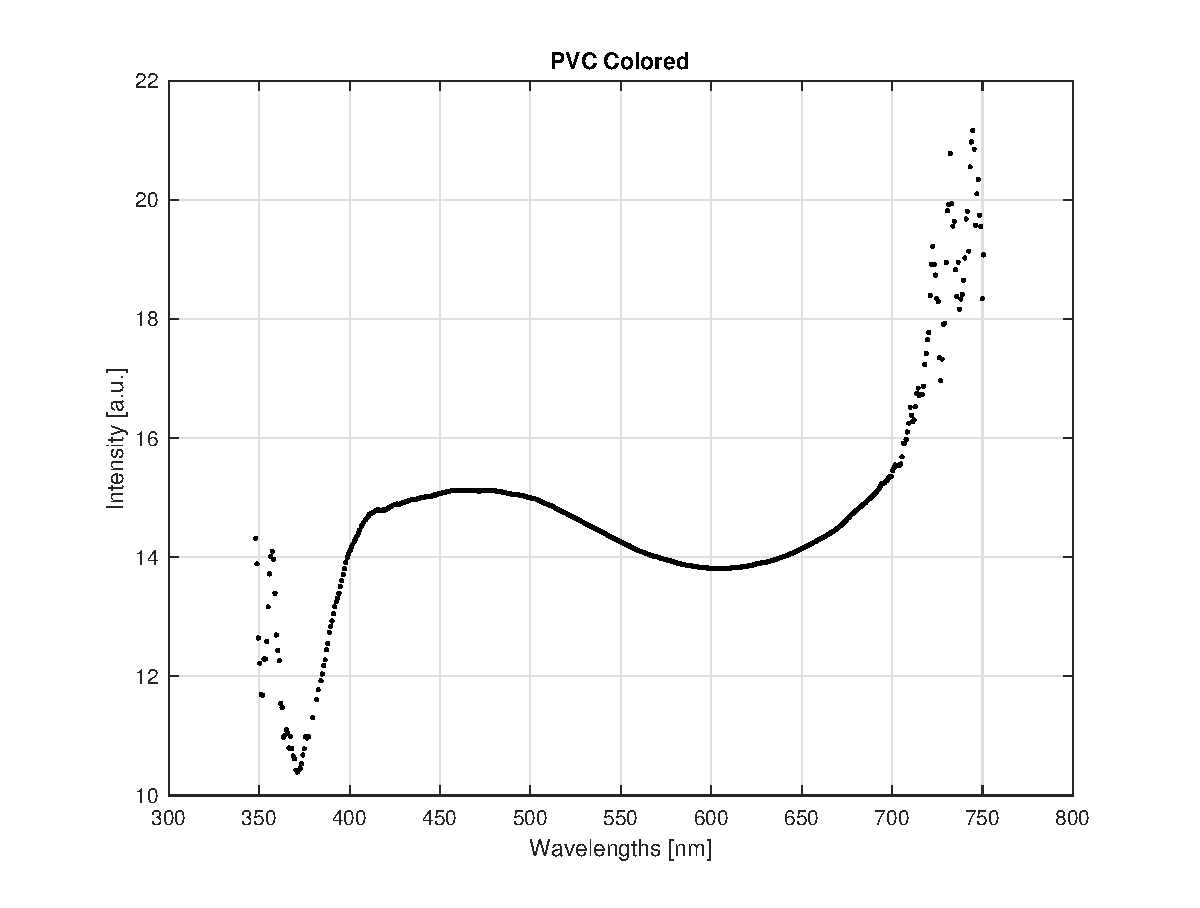
\includegraphics[width = 12cm]{Images/appendix/pvc-pristine-colored.eps}
    \caption{PVC, Pristine, Gray}
    \label{fig:pvc-gray}
\end{figure}

\begin{figure}
    \centering
    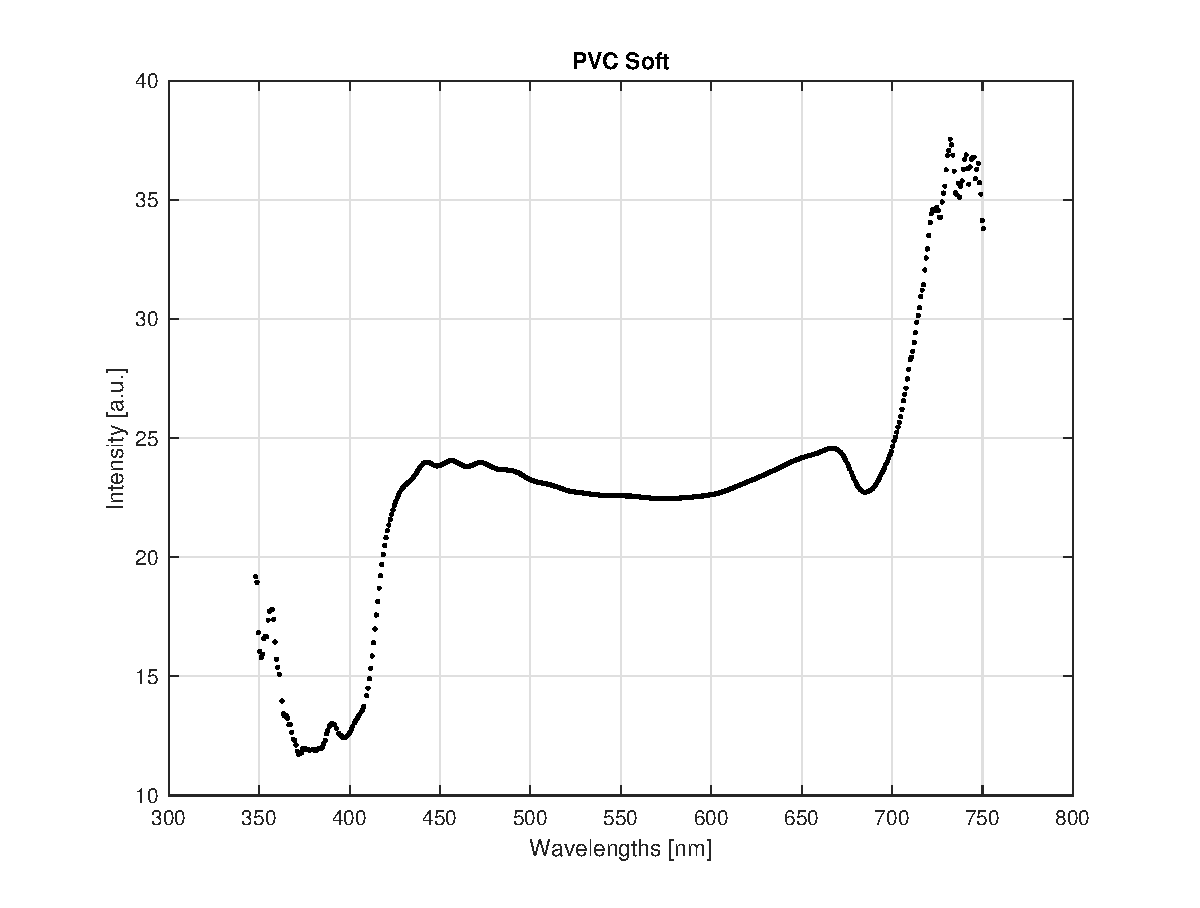
\includegraphics[width = 12cm]{Images/appendix/pvc-soft-pristine-clear.eps}
    \caption{PVC Soft, Pristine, Clear}
    \label{fig:pvc-clear}
\end{figure}

\begin{figure}
    \centering
    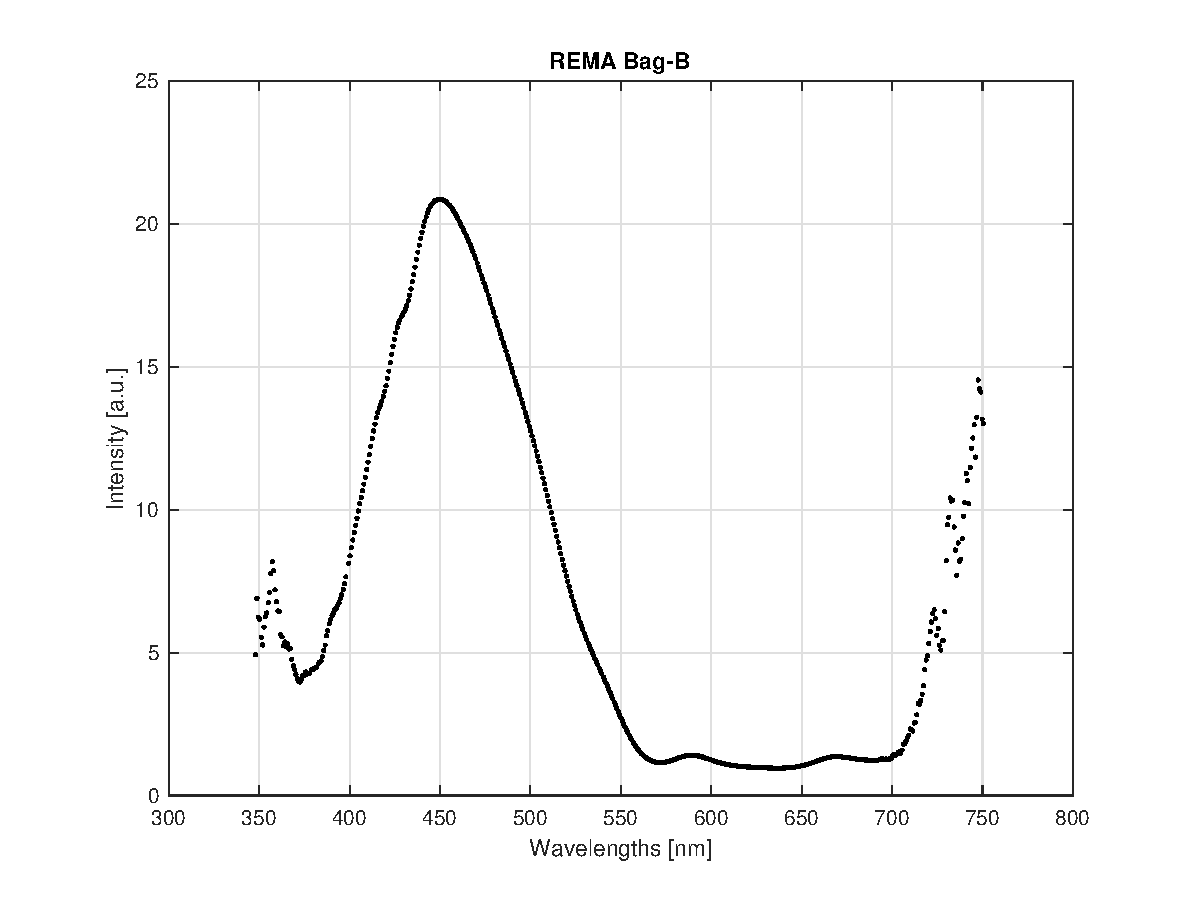
\includegraphics[width = 12cm]{Images/appendix/remablue.eps}
    \caption{REMA Bag, Blue}
    \label{fig:remablue}
\end{figure}

\begin{figure}
    \centering
    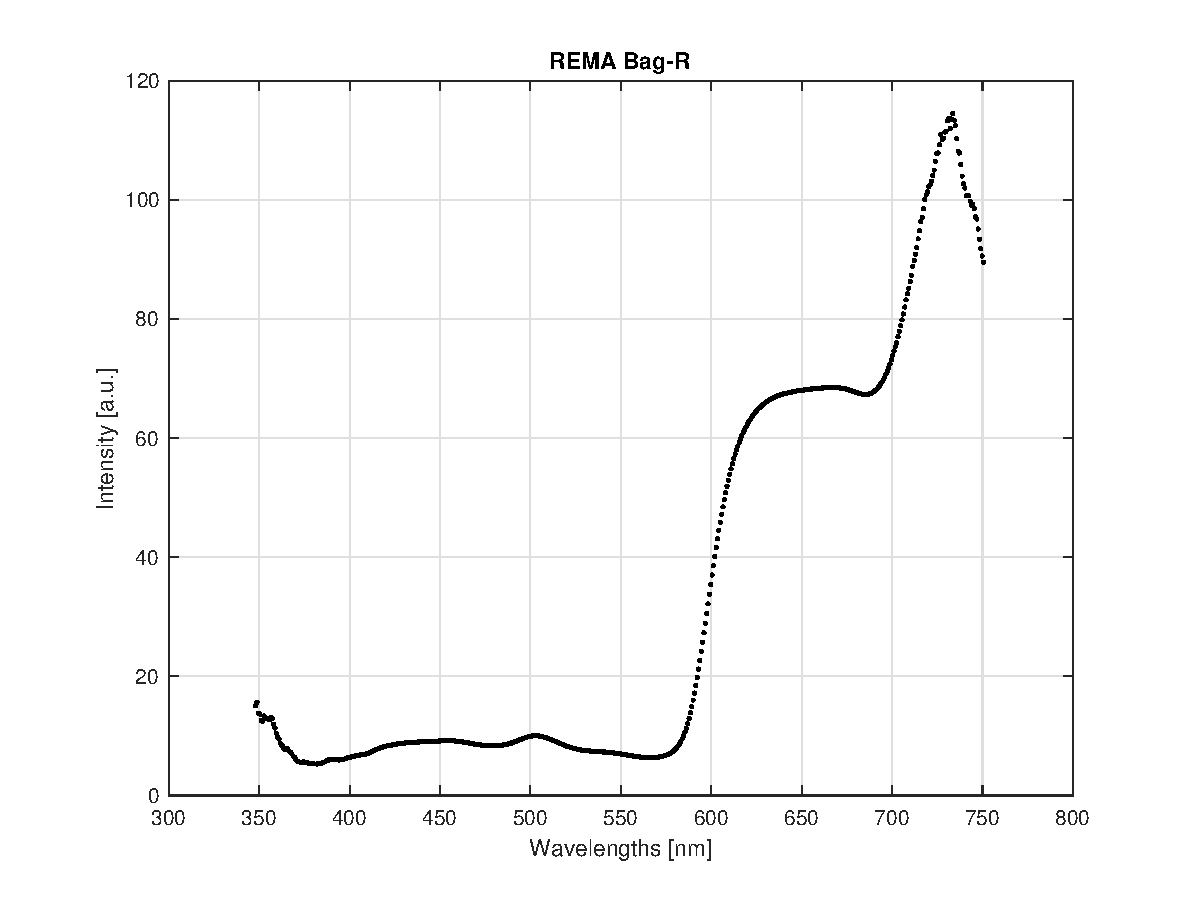
\includegraphics[width = 12cm]{Images/appendix/remared.eps}
    \caption{REMA Bag, Red}
    \label{fig:remared}
\end{figure}

\begin{figure}
    \centering
    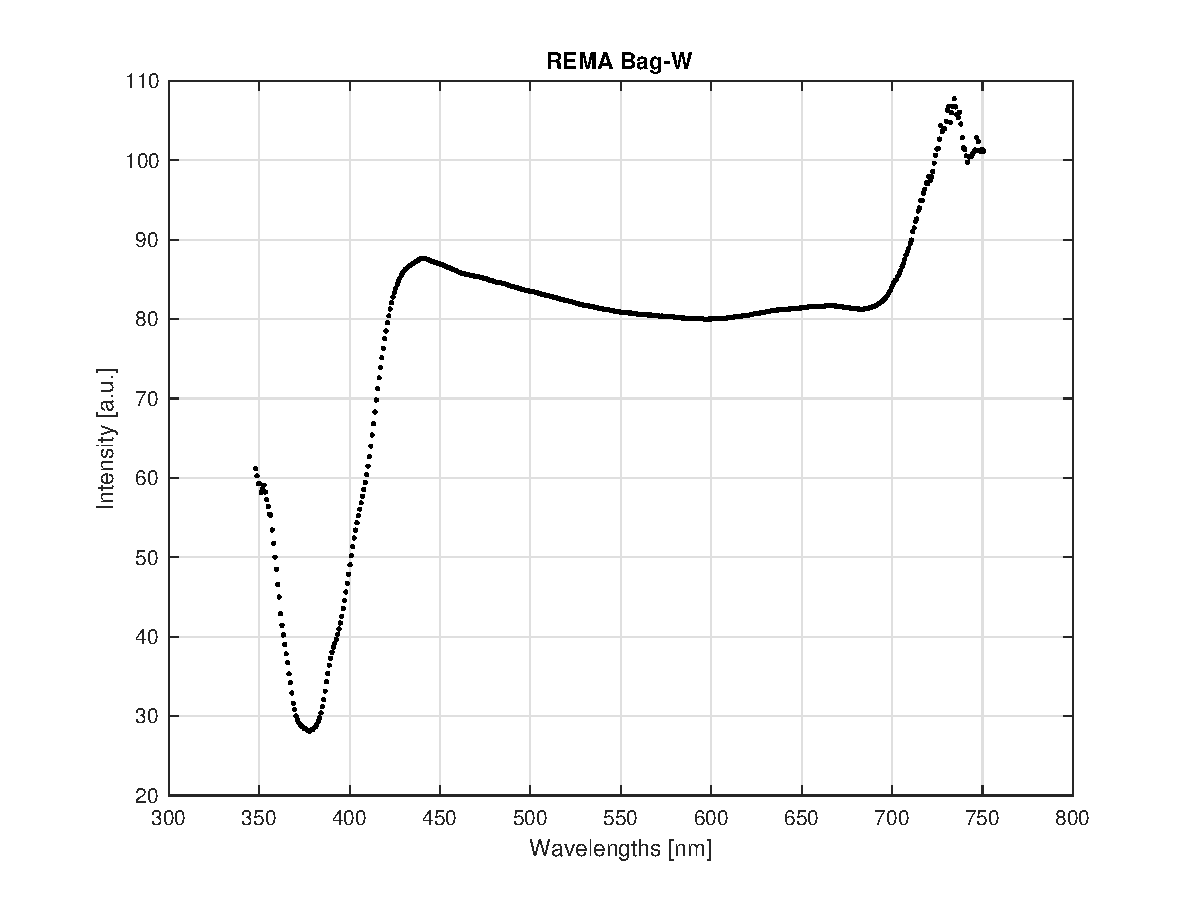
\includegraphics[width = 12cm]{Images/appendix/remawhite.eps}
    \caption{REMA Bag, White}
    \label{fig:remawhite}
\end{figure}

\begin{figure}
    \centering
    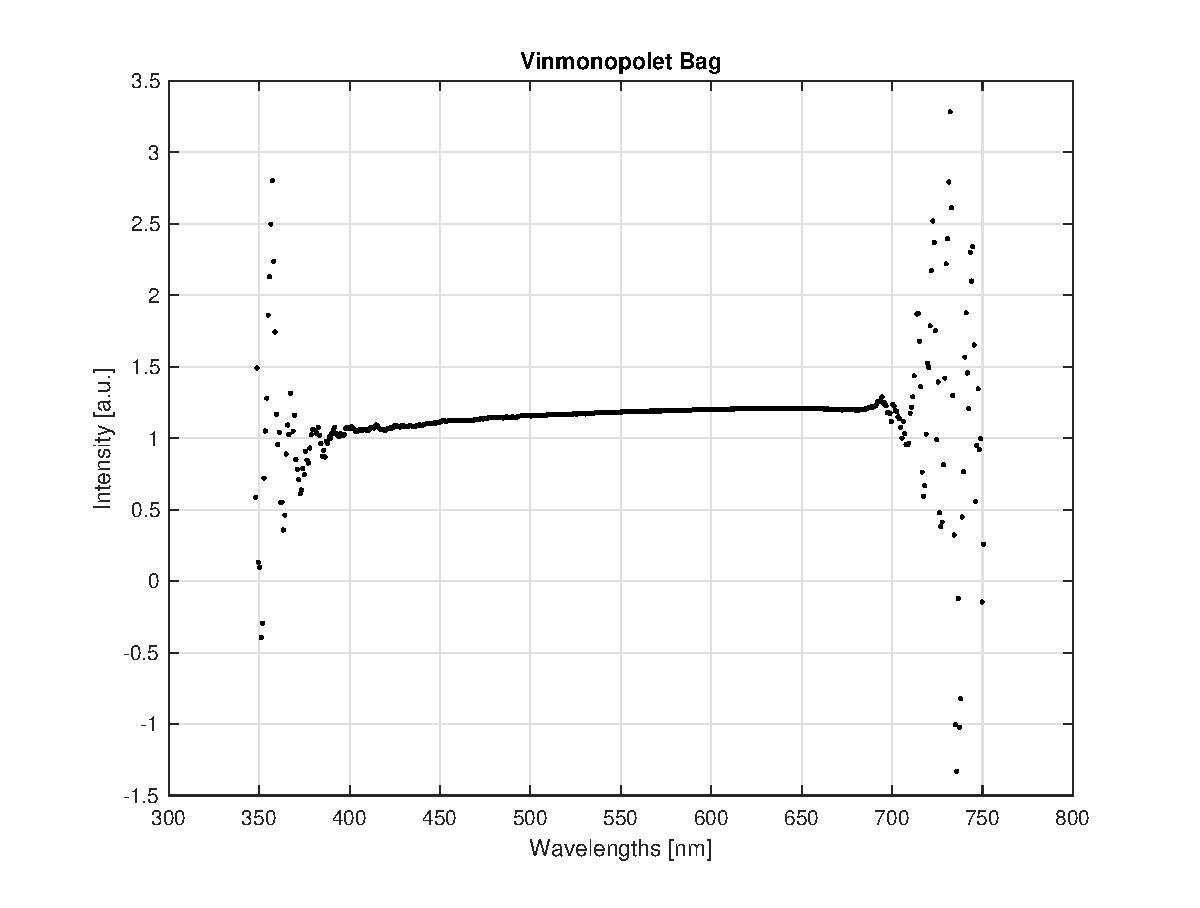
\includegraphics[width = 12cm]{Images/appendix/vinmono.eps}
    \caption{Vinmonopolet Bag, Black}
    \label{fig:vinmono}
\end{figure}





\end{appendices}




